% Provenance (never printed): cycle 4 SVT, "La planete Terre, l'environnement
% et l'action humaine": the relief as a balance between uplift and erosion;
% landforms of the wind, the sea and dissolution; reading a landscape; see
% sources/book1/PROVENANCE.md. Book 1, grade 9, chapter 4.
% Vocabulary guard: owns uplift, dune, cliff, beach and spit (with longshore
% drift), karst (with cave and sinkhole). Landscape and landform are g1's;
% weathering, erosion, deposition, meander and delta are g5's; relief is
% g4's; plates and mountain building are g7's; U-shaped valley and moraine
% are g8's; limestone and the acid test are g6's; acids are the chemistry
% books' (recalled in prose). Contour lines are g9.5's (not used here).
% "Normal fault" and the destruction of mountains are Book 2's.
\chapter{الأشكال التضاريسية}\label{ch:g9:landforms}

على \omterm{def:g1:landscapes-around-us:water}{الساحل} الجنوبي لإنجلترا، تهوي \omterm{def:g9:landforms:cliff}{الجروف} البيضاء للأخوات السبع مباشرة
في \omterm{def:g2:water-on-earth:ocean}{البحر}. وفي السنة العادية تفقد ما يصل إلى متر. وفي شتاء 2014، أخذت
العواصف من \omterm{def:g9:landforms:cliff}{الجروف} عند بيرلينغ غاب، في شهرين، ما تفقده عادةً في سبع
سنوات. وكان طباشير هذه \omterm{def:g9:landforms:cliff}{الجروف} يومًا وحلًا في قاع \omterm{def:g2:water-on-earth:ocean}{بحر}، مكوَّنًا من
القشور الدقيقة لطحالب مجهرية كانت تعيش في مائه. واليوم يقف جدارًا من
\omterm{def:g3:stones-pebbles-sand:rock}{الصخر} الأبيض تقتطع منه الأمواج قليلًا كل سنة. لماذا تتخذ الأرض الأشكال
التي لها، ولماذا يتغير بعضها بهذه
السرعة؟
% ledger: nt:birling-2014, sdnp:birling, nasa:coccoliths

\begin{omfigure}
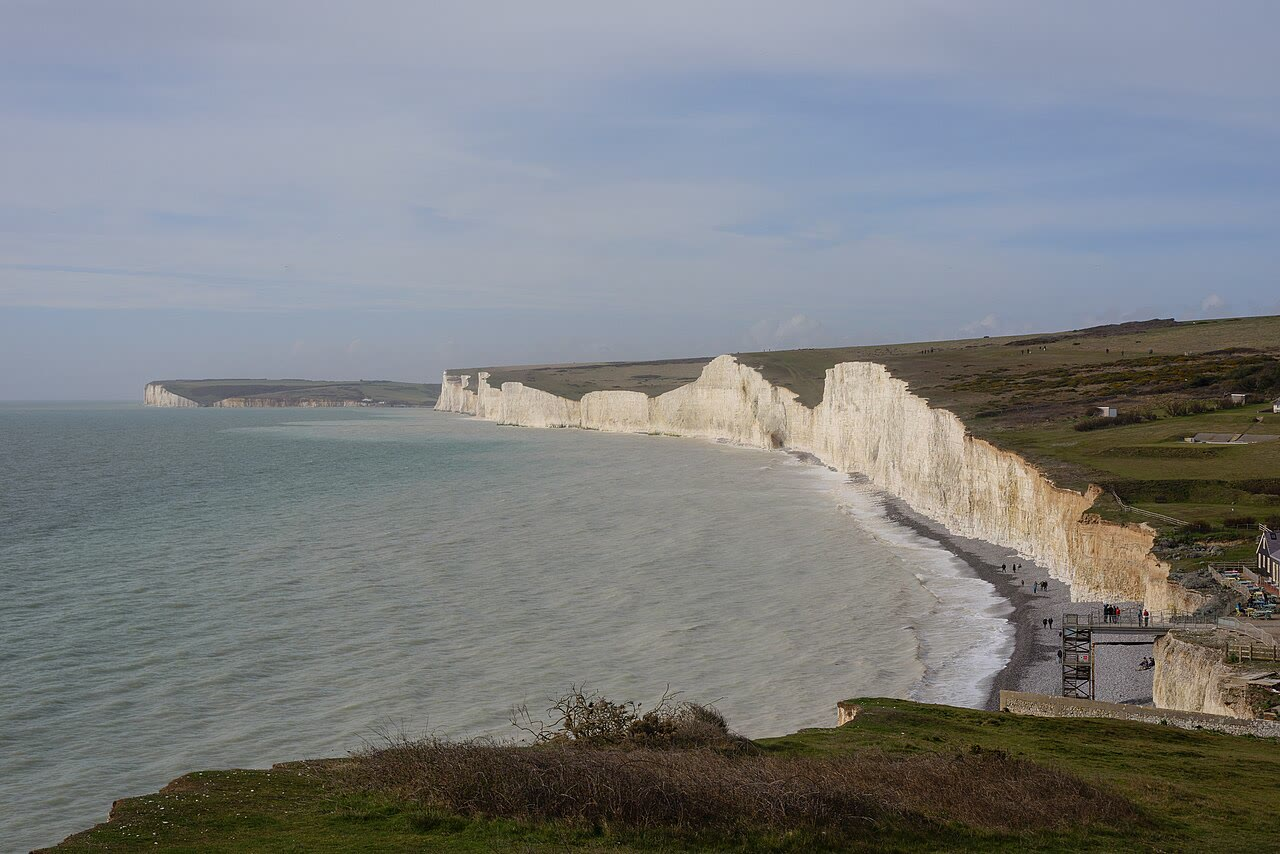
\includegraphics[width=\linewidth]{images/book1/g9-seven-sisters.jpg}

{\small الأخوات السبع، \omterm{def:g9:landforms:cliff}{جروف} طباشيرية على \omterm{def:g1:landscapes-around-us:water}{ساحل} إيست ساسكس (إنجلترا)،
وفي المقدمة بيوت بيرلينغ غاب. \omterm{def:g2:water-on-earth:ocean}{والبحر} يقتطع \omterm{def:g9:landforms:cliff}{الجروف}، وتتساقط \omterm{def:g3:stones-pebbles-sand:rock}{الصخور} في
أي وقت. وعند أقدامها \omterm{def:g9:landforms:beach}{شاطئ} من \omterm{def:g3:stones-pebbles-sand:pebble}{الحصى}. الصورة: أريلد فوغن، 2017
(CC BY-SA 4.0، عبر ويكيميديا
كومنز).}
% ledger: commons:seven-sisters, sdnp:birling
\label{fig:g9:landforms:seven-sisters}
\end{omfigure}

\begin{recall}
\emph{\omterm{def:g1:landscapes-around-us:landform}{الشكل التضاريسي}} شكل واحد من أشكال الأرض: \omterm{def:g1:landscapes-around-us:landform}{تلة}، أو \omterm{def:g1:landscapes-around-us:landform}{وادٍ}، أو \omterm{def:g1:landscapes-around-us:landform}{سهل}، أو
\omterm{def:g9:landforms:cliff}{جرف} (\cref{ch:g1:landscapes-around-us}). \omterm{def:g4:world-physical-map:relief}{والتضاريس} هي شكل الأرض في
\omterm{def:g4:world-physical-map:altitude}{الارتفاع} (\cref{ch:g4:world-physical-map}). \omterm{def:g5:water-shapes-the-land:weathering}{والتجوية} تكسر \omterm{def:g3:stones-pebbles-sand:rock}{الصخر}،
\omterm{def:g5:water-shapes-the-land:erosion}{والتعرية} تبريه وتحمله بعيدًا، \omterm{def:g5:water-shapes-the-land:deposition}{والترسيب} يضعه في مكان آخر
(\cref{ch:g5:water-shapes-the-land}). \omterm{def:g7:plate-tectonics:plate}{والصفائح} تدفع إلى أعلى \omterm{def:g4:world-physical-map:range}{سلاسل جبلية}
حيث تتصادم (\cref{ch:g7:plate-tectonics})؛ \omterm{def:g8:ice-on-earth:glacier}{والأنهار الجليدية} تحفر \omterm{def:g1:landscapes-around-us:landform}{أودية}
على شكل حرف U (\cref{ch:g8:ice-on-earth})؛ والحجر الجيري يفور تحت قطرة
من حمض مخفف (\cref{ch:g6:rocks-and-minerals}). وفي الكيمياء، تتعلم أن
الأحماض تهاجم الحجر الجيري وتطلق ثاني أكسيد الكربون.
\end{recall}

\section{التضاريس: توازن بين الرفع والتعرية}

نوعان من القوى يشكّلان \omterm{def:g4:world-physical-map:relief}{التضاريس}. فمن الداخل، ترفع حركات \omterm{def:g7:plate-tectonics:plate}{الصفائح} الأرض.
ومن الخارج، يبريها الماء والجليد والريح
\omterm{def:g2:water-on-earth:ocean}{والبحر}.

\begin{definition}[الرفع]\label{def:g9:landforms:uplift}
\emph{الرفع}\index{رفع} هو الارتفاع البطيء \omterm{def:g3:stones-pebbles-sand:rock}{لصخور} منطقة ما ولسطح أرضها،
بفعل قوى في باطن الأرض، مثل تصادم
صفيحتين.
\end{definition}

\omterm{def:g9:landforms:uplift}{الرفع} بطيء على سلّم الحياة لكنه سريع على سلّم الأرض. فقد اصطدمت الهند
بآسيا قبل نحو 50~مليون سنة، واكتسبت هضبة التبت، خلف الهيمالايا، معظم
ارتفاعها، نحو \qty{4600}{m}، في آخر 10~ملايين سنة. وهذا في المتوسط
$4600 \div 10^7 = 4.6 \times 10^{-4}$~m، أي نحو \qty{0.5}{mm} في السنة:
أقل من سمك ظفر، لكنه مستمر ملايين
السنين.
% ledger: usgs:himalaya (rate computed in figdata/grade-9/cliff_retreat.py, tibet_rate_mm_yr)

وما إن ترتفع الأرض حتى تهاجمها \omterm{def:g5:water-shapes-the-land:erosion}{التعرية}. فكلما كانت الأرض أعلى وأشد
انحدارًا، حملت \omterm{def:g1:landscapes-around-us:water}{الأنهار} \omterm{def:g8:ice-on-earth:glacier}{والأنهار الجليدية} والانهيارات الصخرية الصخرَ بسرعة
أكبر. \omterm{def:g4:world-physical-map:altitude}{وارتفاع} \omterm{def:g4:world-physical-map:range}{سلسلة جبلية} في أي لحظة هو نتيجة مباراة: ما يرفعه \omterm{def:g9:landforms:uplift}{الرفع}،
ناقص ما تأخذه \omterm{def:g5:water-shapes-the-land:erosion}{التعرية}.

\begin{omfigure}
\begin{tikzpicture}[font=\footnotesize, >={Stealth[length=2mm]}]
  % panel 1: uplift faster than erosion
  \begin{scope}
    \fill[black!13] (0,0) -- (0.5,0) .. controls (1.1,1.0) and (1.5,2.0) .. (1.8,2.2)
      .. controls (2.1,2.0) and (2.5,1.0) .. (3.1,0) -- (3.6,0) -- (3.6,-0.5) -- (0,-0.5) -- cycle;
    \draw[black!60] (0,0) -- (0.5,0) .. controls (1.1,1.0) and (1.5,2.0) .. (1.8,2.2)
      .. controls (2.1,2.0) and (2.5,1.0) .. (3.1,0) -- (3.6,0);
    \draw[black!60, dashed] (0.7,0) .. controls (1.2,0.8) and (1.5,1.5) .. (1.8,1.6)
      .. controls (2.1,1.5) and (2.4,0.8) .. (2.9,0);
    \foreach \x in {1.2,1.8,2.4} \draw[->, omWarm, line width=1.4pt] (\x,-0.45) -- ++(0,1.0);
    \draw[->, omRiver, thick] (2.15,1.6) -- ++(0.35,-0.3);
    \node[align=center, anchor=north] at (1.8,-0.6) {الرفع أسرع من التعرية\\فترتفع التضاريس};
  \end{scope}
  % panel 2: uplift equals erosion
  \begin{scope}[xshift=4.4cm]
    \fill[black!13] (0,0) -- (0.5,0) .. controls (1.1,1.0) and (1.5,1.8) .. (1.8,1.9)
      .. controls (2.1,1.8) and (2.5,1.0) .. (3.1,0) -- (3.6,0) -- (3.6,-0.5) -- (0,-0.5) -- cycle;
    \draw[black!60] (0,0) -- (0.5,0) .. controls (1.1,1.0) and (1.5,1.8) .. (1.8,1.9)
      .. controls (2.1,1.8) and (2.5,1.0) .. (3.1,0) -- (3.6,0);
    \foreach \x in {1.2,1.8,2.4} \draw[->, omWarm, line width=1.4pt] (\x,-0.45) -- ++(0,0.6);
    \draw[->, omRiver, thick] (2.05,1.6) -- ++(0.55,-0.5);
    \draw[->, omRiver, thick] (1.55,1.6) -- ++(-0.55,-0.5);
    \node[align=center, anchor=north] at (1.8,-0.6) {الرفع والتعرية متساويان\\فيبقى الارتفاع كما هو};
  \end{scope}
  % panel 3: no more uplift
  \begin{scope}[xshift=8.8cm]
    \fill[black!13] (0,0) -- (0.4,0) .. controls (1.1,0.5) and (1.5,0.95) .. (1.8,1.0)
      .. controls (2.1,0.95) and (2.5,0.5) .. (3.2,0) -- (3.6,0) -- (3.6,-0.5) -- (0,-0.5) -- cycle;
    \draw[black!60] (0,0) -- (0.4,0) .. controls (1.1,0.5) and (1.5,0.95) .. (1.8,1.0)
      .. controls (2.1,0.95) and (2.5,0.5) .. (3.2,0) -- (3.6,0);
    \draw[black!60, dashed] (0.5,0) .. controls (1.1,1.0) and (1.5,1.8) .. (1.8,1.9)
      .. controls (2.1,1.8) and (2.5,1.0) .. (3.1,0);
    \draw[->, omRiver, thick] (2.05,0.95) -- ++(0.55,-0.5);
    \draw[->, omRiver, thick] (1.55,0.95) -- ++(-0.55,-0.5);
    \node[align=center, anchor=north] at (1.8,-0.6) {توقف الرفع: فالتعرية\\تخفض التضاريس};
  \end{scope}
  % key
  \draw[->, omWarm, line width=1.4pt] (13.2,1.2) -- ++(0,0.6) node[right, black] {الرفع};
  \draw[->, omRiver, thick] (13.2,0.7) -- ++(0.35,-0.3) node[right, black] {التعرية};
  \draw[black!60, dashed] (13.1,-0.1) -- ++(0.5,0) node[right, black] {المقطع السابق};
\end{tikzpicture}

{\small \omterm{def:g4:world-physical-map:relief}{التضاريس} توازن (رسم تخطيطي، ليس بمقياس رسم). يرفع \omterm{def:g9:landforms:uplift}{الرفع} \omterm{def:g3:stones-pebbles-sand:rock}{الصخور}؛
وتحملها \omterm{def:g5:water-shapes-the-land:erosion}{التعرية} إلى \omterm{def:g1:landscapes-around-us:landform}{الأودية} \omterm{def:g2:water-on-earth:ocean}{والبحر}. وتواصل السلسلة النمو ما دام \omterm{def:g9:landforms:uplift}{الرفع}
غالبًا؛ وحين تكف \omterm{def:g7:plate-tectonics:plate}{الصفائح} عن الدفع، تبريها \omterm{def:g5:water-shapes-the-land:erosion}{التعرية} ببطء حتى تصير
تلالًا.}
\label{fig:g9:landforms:balance}
\end{omfigure}

\omterm{def:g1:landscapes-around-us:water}{الأنهار} (\cref{ch:g5:water-shapes-the-land}) \omterm{def:g8:ice-on-earth:glacier}{والأنهار الجليدية}
(\cref{ch:g8:ice-on-earth}) هي النحّاتة الكبرى \omterm{def:g1:landscapes-around-us:landform}{للجبال}. وبقية هذا الفصل
تتبع ثلاثة عوامل أخرى، تصنع أشكالًا تضاريسية خاصة بها: الريح، \omterm{def:g2:water-on-earth:ocean}{والبحر}،
والماء الذي يذيب \omterm{def:g3:stones-pebbles-sand:rock}{الصخر}.

\section{أشكال تضاريسية تصنعها الريح: الكثبان}

حيث تقل النباتات، ويكثر \omterm{def:g3:stones-pebbles-sand:sand}{الرمل} المفكك وتشتد الريح، تستطيع الريح أن ترفع
\omterm{def:g3:stones-pebbles-sand:sand}{الرمل} وتكومه تلالًا: في \omterm{def:g5:weather-and-climate:desert}{الصحارى}، وخلف \omterm{def:g9:landforms:beach}{الشواطئ}
الرملية.
% ledger: nps:aeolian

\begin{definition}[الكثيب]\label{def:g9:landforms:dune}
\emph{الكثيب}\index{كثيب} كومة أو حافة من \omterm{def:g3:stones-pebbles-sand:sand}{الرمل} المفكك كوّمتها الريح.
منحدره المواجه للريح طويل لطيف؛ وجانبه البعيد،
\emph{وجه الانزلاق}\index{وجه انزلاق}، قصير شديد الانحدار.
\end{definition}
% ledger: nps:aeolian, nmt:barchan

\omterm{def:g9:landforms:dune}{الكثيب} يتحرك. فالريح تدحرج الحبيبات وتقفزها صعودًا على المنحدر اللطيف؛
وعند الذروة تتكوم حتى تصير الكومة شديدة الانحدار، فينزلق انهيار صغير من
\omterm{def:g3:stones-pebbles-sand:sand}{الرمل} على \omterm{def:g9:landforms:dune}{وجه الانزلاق}. وحبيبة بعد حبيبة، يُؤخذ \omterm{def:g3:stones-pebbles-sand:sand}{الرمل} من الجانب المواجه
للريح ويوضع على الجانب البعيد، فيزحف \omterm{def:g9:landforms:dune}{الكثيب} كله مع الريح دون أن يُرفع
أبدًا. ونادرًا ما تقف \omterm{def:g9:landforms:dune}{الكثبان} منفردة: فهي تغطي حقولًا
كاملة.
% ledger: nmt:barchan, nps:aeolian

وحيث تهب الريح دائمًا من الاتجاه نفسه ولا يكون \omterm{def:g3:stones-pebbles-sand:sand}{الرمل} وفيرًا جدًا، تتخذ
\omterm{def:g9:landforms:dune}{الكثبان} شكل هلال، هو \emph{البرخان}: أنفه المستدير يواجه الريح وقرناه
يشيران مع اتجاه الريح. والقرنان يحويان \omterm{def:g3:stones-pebbles-sand:sand}{رملًا} أقل من الوسط، فيتحركان
أسرع ويمتدان أمام \omterm{def:g9:landforms:dune}{الكثيب}.
% ledger: nmt:barchan

\begin{omfigure}
\begin{tikzpicture}[font=\footnotesize, >={Stealth[length=2mm]}]
  % plan view
  \fill[yellow!25!orange!20] (3.4,1.3) .. controls (1.0,1.3) and (0.2,0.6) .. (0.2,0)
     .. controls (0.2,-0.6) and (1.0,-1.3) .. (3.4,-1.3)
     .. controls (2.4,-0.9) and (1.8,-0.5) .. (1.8,0)
     .. controls (1.8,0.5) and (2.4,0.9) .. (3.4,1.3) -- cycle;
  \fill[orange!45] (3.4,1.3) .. controls (2.4,0.9) and (1.8,0.5) .. (1.8,0)
     .. controls (1.8,-0.5) and (2.4,-0.9) .. (3.4,-1.3)
     .. controls (2.1,-0.8) and (1.45,-0.45) .. (1.45,0)
     .. controls (1.45,0.45) and (2.1,0.8) .. (3.4,1.3) -- cycle;
  \draw[black!60] (3.4,1.3) .. controls (1.0,1.3) and (0.2,0.6) .. (0.2,0)
     .. controls (0.2,-0.6) and (1.0,-1.3) .. (3.4,-1.3)
     .. controls (2.4,-0.9) and (1.8,-0.5) .. (1.8,0)
     .. controls (1.8,0.5) and (2.4,0.9) .. (3.4,1.3);
  \draw[black, thick] (3.4,1.3) .. controls (2.1,0.8) and (1.45,0.45) .. (1.45,0)
     .. controls (1.45,-0.45) and (2.1,-0.8) .. (3.4,-1.3);
  \foreach \y in {-0.8,0,0.8} \draw[->, omRiver, thick] (-1.3,\y) -- ++(1.1,0);
  \node[above] at (-0.75,0.85) {الريح};
  \node[anchor=west] at (3.5,1.35) {قرن};
  \node[anchor=west] at (3.5,-1.35) {قرن};
  \draw[black!70] (1.75,0.25) -- (2.9,0.35) node[anchor=west, align=left, black] {وجه الانزلاق\\شديد الانحدار};
  \draw[black!70] (0.75,-0.2) -- (0.6,-1.6) node[anchor=north, align=center, black] {منحدر لطيف\\مواجه للريح};
  \draw[black!70] (1.47,-0.3) -- (2.4,-1.75) node[anchor=north, black] {الذروة};
  \node[anchor=south, font=\footnotesize\bfseries] at (1.4,1.6) {منظر من أعلى};
  % profile
  \begin{scope}[xshift=7.2cm, yshift=-0.8cm]
    \draw[black!60] (-0.4,0) -- (5.6,0);
    \fill[yellow!25!orange!20] (0,0) -- (3.0,1.2) -- (3.6,0) -- cycle;
    \draw[black!70] (0,0) -- (3.0,1.2) -- (3.6,0);
    \fill[orange!45] (3.0,1.2) -- (3.6,0) -- (3.3,0) -- cycle;
    \draw[black!50, dashed] (0.8,0) -- (3.8,1.2) -- (4.4,0);
    \draw[->, black!70] (0.5,0.35) .. controls (0.75,0.65) .. (1.0,0.45);
    \draw[->, black!70] (1.0,0.55) .. controls (1.25,0.85) .. (1.5,0.65);
    \draw[->, black!70] (1.5,0.75) .. controls (1.75,1.05) .. (2.0,0.85);
    \draw[->, black!70] (2.0,0.95) .. controls (2.25,1.25) .. (2.5,1.05);
    \draw[->, thick, black!80] (3.15,1.05) -- (3.45,0.35);
    \foreach \y in {1.6,2.1} \draw[->, omRiver, thick] (-0.8,\y) -- ++(1.1,0);
    \node[above] at (-0.25,2.1) {الريح};
    \draw[->, thick] (4.5,0.6) -- ++(0.7,0) node[right, align=left] {الكثيب\\يتحرك};
    \node[align=center, anchor=north] at (1.2,-0.1) {الحبيبات تقفز صعودًا\\على المنحدر اللطيف};
    \node[align=center, anchor=north west] at (2.9,-0.1) {ثم تنزلق على\\وجه الانزلاق};
    \node[anchor=south, font=\footnotesize\bfseries] at (2.2,2.3) {منظر جانبي};
  \end{scope}
\end{tikzpicture}

{\small \omterm{def:g9:landforms:dune}{كثيب} هلالي، أو برخان (رسم تخطيطي). من أعلى، يشير قرناه مع اتجاه
الريح. ومن الجانب، تصعد الحبيبات المنحدر اللطيف المواجه للريح وتنزلق على
\omterm{def:g9:landforms:dune}{وجه الانزلاق} الشديد الانحدار: فيتحرك \omterm{def:g9:landforms:dune}{الكثيب} مع الريح (الخط المتقطع:
\omterm{def:g9:landforms:dune}{الكثيب} بعد قليل).}
% ledger: nmt:barchan, nps:aeolian
\label{fig:g9:landforms:barchan}
\end{omfigure}

وبأي سرعة؟ في حقل \omterm{def:g9:landforms:dune}{كثبان} الجبس في وايت ساندز، في نيومكسيكو، تتحرك
\omterm{def:g9:landforms:dune}{الكثبان} الصغيرة التي تتكوّن عند طرفه المواجه للريح، وارتفاعها بضعة أمتار،
حتى \qty{6}{m} في السنة؛ وبعد ذلك بقليل، حين يبلغ ارتفاعها 6 إلى
\qty{10}{m}، تتحرك نحو \qty{3}{m} في السنة. وكلما زاد \omterm{def:g3:stones-pebbles-sand:sand}{الرمل} في \omterm{def:g9:landforms:dune}{الكثيب}،
أبطأ سيره. والبرخانات التي تدفعها رياح قوية قد تقطع أكثر من
\qty{100}{m} في السنة، وهذا يكفي لطمر طريق أو حقل.
% ledger: nps:whsa-migration, nmt:barchan

\begin{omfigure}
\begin{minipage}[c]{0.5\linewidth}\centering
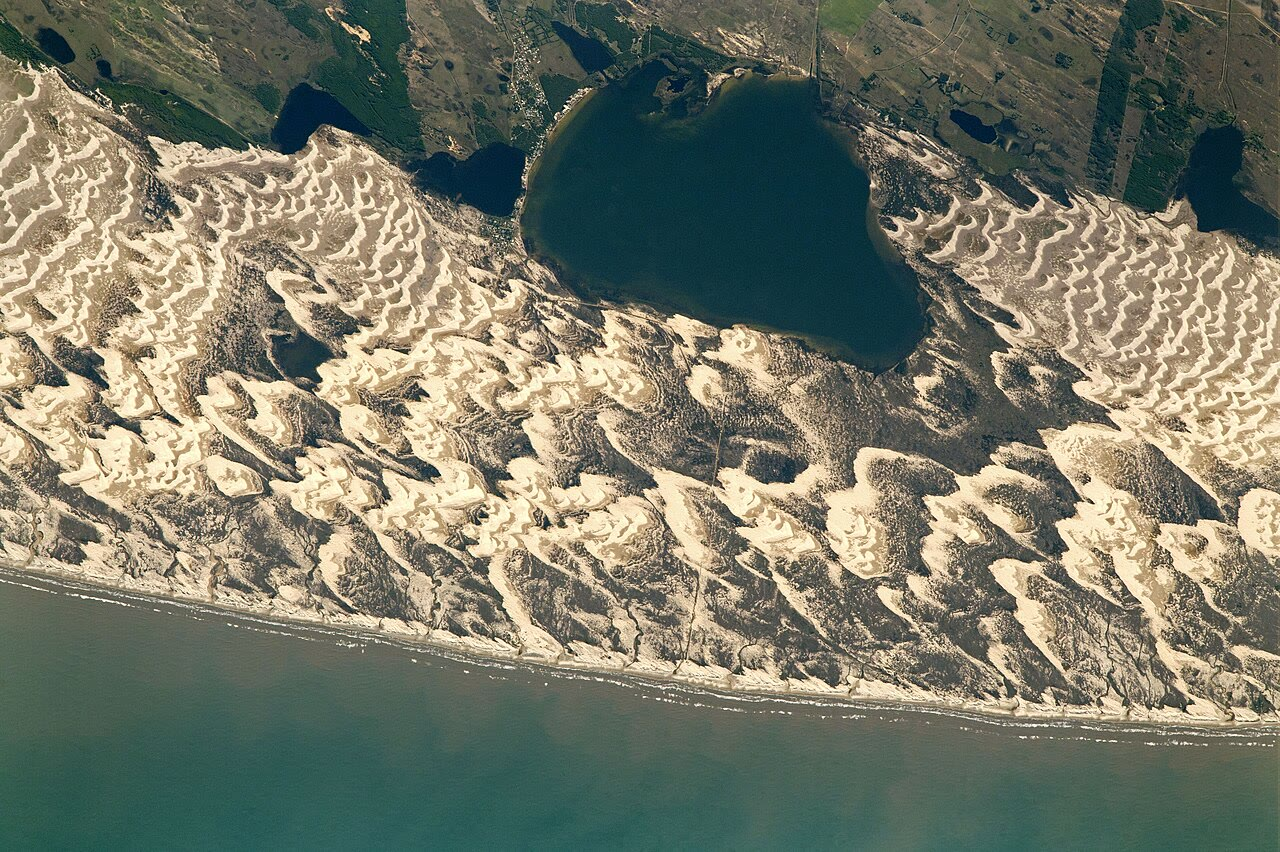
\includegraphics[width=\linewidth]{images/book1/g9-barchans.jpg}
\end{minipage}\hfill
\begin{minipage}[c]{0.46\linewidth}\raggedright
{\small \omterm{def:g9:landforms:dune}{كثبان} هلالية الشكل على \omterm{def:g1:landscapes-around-us:water}{ساحل} الأطلسي في جنوب البرازيل، صوّرها
رائد فضاء من محطة الفضاء الدولية في عام 2017. \omterm{def:g1:landscapes-around-us:water}{والبحيرة} الداكنة، لاغوا
دوس باروس، طولها نحو \qty{4.5}{km}. ويأتي \omterm{def:g3:stones-pebbles-sand:sand}{الرمل} من \omterm{def:g9:landforms:beach}{الشاطئ}، في أسفل
الصورة. ناسا (ملك عام، عبر ويكيميديا
كومنز).}
\end{minipage}
% ledger: commons:iss-barchans
\label{fig:g9:landforms:barchans-photo}
\end{omfigure}

على \omterm{def:g1:landscapes-around-us:water}{الساحل}، يحمي خط من \omterm{def:g9:landforms:dune}{الكثبان} خلف \omterm{def:g9:landforms:beach}{الشاطئ} الأرض التي وراءه من أمواج
العواصف. والنباتات التي تنمو على \omterm{def:g9:landforms:dune}{الكثبان} تمسك \omterm{def:g3:stones-pebbles-sand:sand}{الرمل} بجذورها: وحيث تُداس
أو تُزال، تعود الريح فتأخذ \omterm{def:g3:stones-pebbles-sand:sand}{الرمل}.
% ledger: nps:aeolian

\section{أشكال تضاريسية يصنعها البحر}

\subsection{الجروف}

\begin{definition}[الجرف]\label{def:g9:landforms:cliff}
\emph{الجرف}\index{جرف} واجهة صخرية شديدة الانحدار أو قائمة. وعلى
\omterm{def:g1:landscapes-around-us:water}{الساحل}، تقتطع الأمواج الجرف، فتهاجم قاعدته وتجعله يتراجع نحو
اليابسة.
\end{definition}

تقذف الأمواج الماء \omterm{def:g3:stones-pebbles-sand:sand}{والرمل} \omterm{def:g3:stones-pebbles-sand:pebble}{والحصى} على قاعدة \omterm{def:g9:landforms:cliff}{الجرف}. وشيئًا فشيئًا تحفر
تجويفًا في أسفله، هو \emph{الحزّ}، بين مستويي الجزر والمد. فيبرز \omterm{def:g3:stones-pebbles-sand:rock}{الصخر}
الذي فوقه؛ ويزيده \omterm{def:g4:clouds-rain-snow:precipitation}{المطر} والصقيع ضعفًا. وذات يوم يسقط البروز. فتكسر
الأمواج الكتل الساقطة وتحملها بعيدًا، ويبدأ الهجوم من جديد على واجهة
جديدة، أبعد قليلًا نحو اليابسة. ويترك \omterm{def:g9:landforms:cliff}{الجرف} وراءه رفًا مستويًا من
\omterm{def:g3:stones-pebbles-sand:rock}{الصخر}، هو \emph{مصطبة نحت الأمواج}\index{مصطبة نحت الأمواج}، التي تظهر
عند الجزر.
% ledger: nt:birling-2014, sdnp:birling

\omterm{def:g3:stones-pebbles-sand:rock}{الصخور} الطرية تتراجع أسرع. ففي بيرلينغ غاب، تفقد \omterm{def:g9:landforms:cliff}{الجروف} الطباشيرية ما
يصل إلى نحو متر في السنة؛ لكن التراجع يأتي قفزات، انهيارًا بعد انهيار،
وقد يأخذ شتاء عاصف تراجع سنوات دفعة واحدة. وفي عام 1999، نُقلت المنارة
القديمة بيل تو، المبنية عام 1832 فوق \omterm{def:g9:landforms:cliff}{الجروف} القريبة، \qty{17}{m} إلى
الوراء بعيدًا عن الحافة، قطعةً واحدة، لأن \omterm{def:g9:landforms:cliff}{الجرف} كان يقترب منها
كثيرًا.
% ledger: sdnp:birling, nt:birling-2014

\begin{omfigure}
\begin{tikzpicture}[font=\footnotesize, >={Stealth[length=2mm]}]
  % panel 1: the notch
  \begin{scope}
    \fill[omSea!45] (0,-0.1) rectangle (1.8,0.75);
    \fill[omSea!45] (1.8,0.35) -- (2.25,0.55) -- (1.8,0.95) -- cycle;
    \fill[black!8] (1.6,-0.1) -- (1.8,0.25) -- (1.8,0.35) -- (2.25,0.55) -- (1.8,0.95) -- (1.8,2.4) -- (3.6,2.4) -- (3.6,-0.6) -- (0,-0.6) -- (0,-0.1) -- cycle;
    \draw[black!70] (0,-0.1) -- (1.6,-0.1) -- (1.8,0.25) -- (1.8,0.35) -- (2.25,0.55) -- (1.8,0.95) -- (1.8,2.4) -- (3.6,2.4);
    \foreach \y in {0.8,1.3,1.8} \draw[black!25] (1.8,\y) -- (3.6,\y);
    \fill[green!35!black!50] (1.8,2.4) rectangle (3.6,2.5);
    \draw[->, omSea!80!black, thick] (0.4,0.6) -- (1.6,0.6);
    \node[anchor=south, align=center] at (0.9,0.8) {الأمواج};
    \draw[black!70] (2.15,0.55) -- (2.9,1.0) node[anchor=west, fill=white, inner sep=1pt] {الحزّ};
    \node[anchor=north, align=center] at (1.8,-0.7) {\foreignlanguage{arabic}{1. الأمواج تحفر}\\حزًّا};
    \node[anchor=south, font=\footnotesize] at (2.7,2.5) {طباشير};
  \end{scope}
  % panel 2: collapse
  \begin{scope}[xshift=4.6cm]
    \fill[omSea!45] (0,-0.1) rectangle (2.2,0.75);
    \fill[black!8] (2.0,-0.1) -- (2.2,0.25) -- (2.25,2.4) -- (3.6,2.4) -- (3.6,-0.6) -- (0,-0.6) -- (0,-0.1) -- cycle;
    \draw[black!70] (0,-0.1) -- (2.0,-0.1) -- (2.2,0.25) -- (2.25,2.4) -- (3.6,2.4);
    \draw[black!50, dashed] (1.8,0.95) -- (1.8,2.4) -- (2.25,2.4);
    \foreach \y in {0.8,1.3,1.8} \draw[black!25] (2.25,\y) -- (3.6,\y);
    \fill[green!35!black!50] (2.25,2.4) rectangle (3.6,2.5);
    \foreach \x/\y/\s in {1.25/0.05/0.28, 1.6/0.1/0.22, 1.95/0.3/0.3, 1.45/0.35/0.18}
      \fill[black!20, draw=black!60] (\x,\y) rectangle ++(\s,\s*0.8);
    \node[anchor=north, align=center] at (1.8,-0.7) {\foreignlanguage{arabic}{2. البروز}\\يسقط};
  \end{scope}
  % panel 3: retreat and platform
  \begin{scope}[xshift=9.2cm]
    \fill[omSea!45] (0,0.2) rectangle (2.8,0.75);
    \fill[black!8] (0,0.0) -- (2.6,0.2) -- (2.8,0.3) -- (2.85,2.4) -- (4.0,2.4) -- (4.0,-0.6) -- (0,-0.6) -- cycle;
    \draw[black!70] (0,0.0) -- (2.6,0.2) -- (2.8,0.3) -- (2.85,2.4) -- (4.0,2.4);
    \foreach \y in {0.8,1.3,1.8} \draw[black!25] (2.85,\y) -- (4.0,\y);
    \fill[green!35!black!50] (2.85,2.4) rectangle (4.0,2.5);
    \draw[black!50, dashed] (1.4,0.12) -- (1.4,2.4);
    \draw[black!50, dashed] (2.1,0.16) -- (2.1,2.4);
    \draw[<-, thick] (2.8,1.6) -- (1.5,1.6);
    \node[anchor=south, align=center] at (1.4,2.45) {واجهات الجرف القديمة};
    \node[anchor=north, align=center] at (2.0,-0.7) {\foreignlanguage{arabic}{3. مصطبة نحت الأمواج}\\تنكشف عند الجزر};
  \end{scope}
\end{tikzpicture}

{\small كيف يتراجع \omterm{def:g9:landforms:cliff}{جرف} بحري (رسم تخطيطي، ليس بمقياس رسم). (1) تحفر
الأمواج حزًّا عند قاعدة \omterm{def:g9:landforms:cliff}{الجرف}. (2) يسقط \omterm{def:g3:stones-pebbles-sand:rock}{الصخر} البارز؛ فتكسر الأمواج
الكتل وتحملها بعيدًا. (3) تتكرر الدورة: فيتحرك \omterm{def:g9:landforms:cliff}{الجرف} نحو اليابسة ويترك
أمامه مصطبة صخرية مستوية.}
% ledger: nt:birling-2014, sdnp:birling
\label{fig:g9:landforms:cliff-retreat}
\end{omfigure}

\begin{safety}
قد تنهار حافة \omterm{def:g9:landforms:cliff}{الجرف} في أي لحظة، وتسقط \omterm{def:g3:stones-pebbles-sand:rock}{الصخور} من الواجهة دون إنذار.
وتُراقب \omterm{def:g9:landforms:cliff}{الجروف} من مسافة آمنة، بعيدًا عن الحافة في الأعلى وبعيدًا عن
القاعدة على \omterm{def:g9:landforms:beach}{الشاطئ}، ويُغادَر \omterm{def:g9:landforms:beach}{الشاطئ} الذي تحت \omterm{def:g9:landforms:cliff}{الجروف} قبل أن يأتي
المد.
\end{safety}
% ledger: nt:birling-2014, sdnp:birling

\subsection{الشواطئ والألسنة الرملية}

\omterm{def:g3:stones-pebbles-sand:sand}{الرمل} \omterm{def:g3:stones-pebbles-sand:pebble}{والحصى} المقتطعان من \omterm{def:g9:landforms:cliff}{الجروف}، وما تنزله \omterm{def:g1:landscapes-around-us:water}{الأنهار}، لا يبقيان حيث
يسقطان: فالأمواج تفرزهما وتنقلهما على طول \omterm{def:g1:landscapes-around-us:water}{الساحل}.

\begin{definition}[الشاطئ والانجراف الساحلي واللسان الرملي]\label{def:g9:landforms:beach}
\emph{الشاطئ}\index{شاطئ} شريط من \omterm{def:g3:stones-pebbles-sand:sand}{الرمل} أو \omterm{def:g3:stones-pebbles-sand:pebble}{الحصى} كوّمته الأمواج على طول
خط \omterm{def:g1:landscapes-around-us:water}{الساحل}. وحين تبلغ الأمواج خط \omterm{def:g1:landscapes-around-us:water}{الساحل} بزاوية، تدفع كل موجة الحبيبات
صعودًا على الشاطئ بتلك الزاوية ويعود الماء مباشرة إلى أسفل المنحدر:
فتتعرج الحبيبات على طول \omterm{def:g1:landscapes-around-us:water}{الساحل}. وهذه الحركة \omterm{def:g3:stones-pebbles-sand:sand}{للرمل} \omterm{def:g3:stones-pebbles-sand:pebble}{والحصى} على طول خط
\omterm{def:g1:landscapes-around-us:water}{الساحل} هي \emph{الانجراف الساحلي}\index{انجراف ساحلي}.
و\emph{اللسان الرملي}\index{لسان رملي} حافة طويلة ضيقة من \omterm{def:g3:stones-pebbles-sand:sand}{الرمل} أو \omterm{def:g3:stones-pebbles-sand:pebble}{الحصى}
يبنيها الانجراف الساحلي، متصلة باليابسة من طرف، وتمتد في \omterm{def:g2:water-on-earth:ocean}{البحر} حيث
ينعطف \omterm{def:g1:landscapes-around-us:water}{الساحل}.
\end{definition}
% ledger: noaa:longshore

وحيث ينحني \omterm{def:g1:landscapes-around-us:water}{الساحل}، عند مدخل خليج أو \omterm{def:g5:water-shapes-the-land:source-mouth}{مصب} \omterm{def:g1:landscapes-around-us:water}{نهر}، يواصل الانجراف سيره في
الاتجاه نفسه ويلقي حمولته في الماء الأهدأ: فينمو \omterm{def:g9:landforms:beach}{الشاطئ} في \omterm{def:g2:water-on-earth:ocean}{البحر} لسانًا
رمليًا. وكثيرًا ما يلتف طرفه نحو الداخل، تثنيه أمواج آتية من اتجاهات
أخرى. وخلف اللسان، في مأمن من الأمواج، يترسب \omterm{def:g3:stones-pebbles-sand:sand}{الوحل} وتنمو المستنقعات
الملحية.
% ledger: noaa:longshore

\begin{omfigure}
\begin{tikzpicture}[font=\footnotesize, >={Stealth[length=2mm]}]
  % sea
  \fill[omSea!40] (0,0) rectangle (11,2.3);
  % land with a bay
  \fill[green!25!black!20] (0,2.3) -- (6,2.3) .. controls (6.3,3.0) and (7.0,3.5) .. (8.0,3.5)
     .. controls (9.0,3.5) and (9.3,2.8) .. (9.5,2.3) -- (11,2.3) -- (11,4.6) -- (0,4.6) -- cycle;
  % calm water of the bay
  \fill[omSea!20] (6,2.3) .. controls (6.3,3.0) and (7.0,3.5) .. (8.0,3.5)
     .. controls (9.0,3.5) and (9.3,2.8) .. (9.5,2.3) -- cycle;
  % salt marsh
  \fill[green!50!black!35] (6.15,2.55) .. controls (6.6,3.1) and (7.3,3.2) .. (7.9,3.0)
     .. controls (7.6,2.7) and (7.0,2.6) .. (6.15,2.55) -- cycle;
  \node[anchor=west, font=\scriptsize] at (6.5,3.85) {مستنقع ملحي};
  \draw[black!60] (6.9,3.75) -- (7.0,2.95);
  % river
  \draw[omRiver, line width=1.2pt] (8.6,4.6) .. controls (8.5,4.0) and (8.3,3.7) .. (8.3,3.48);
  \node[anchor=west, font=\scriptsize] at (8.65,4.25) {نهر};
  % beach
  \fill[yellow!40!orange!35] (0,1.85) rectangle (6,2.3);
  % spit
  \fill[yellow!40!orange!35] (5.9,1.85) .. controls (7.0,1.95) and (7.8,2.0) .. (8.35,2.1)
     .. controls (8.6,2.2) and (8.6,2.5) .. (8.4,2.65) -- (8.25,2.55)
     .. controls (8.35,2.45) and (8.3,2.35) .. (8.15,2.32)
     .. controls (7.5,2.28) and (6.8,2.3) .. (6.0,2.3) -- cycle;
  \draw[black!60] (0,2.3) -- (6,2.3) .. controls (6.3,3.0) and (7.0,3.5) .. (8.0,3.5)
     .. controls (9.0,3.5) and (9.3,2.8) .. (9.5,2.3) -- (11,2.3);
  % waves arriving at an angle
  \foreach \x in {0.9,2.0,3.1,4.2} \draw[omSea!70!black, line width=0.5pt] (\x,1.15) -- ++(-35:1.1);
  \draw[->, omSea!70!black, thick] (0.6,0.3) -- ++(55:1.2) node[pos=0.15, left, black] {الأمواج};
  % zigzag of a pebble
  \draw[->, black, thick] (1.0,1.9) -- (1.35,2.2) -- (1.35,1.9) -- (1.7,2.2) -- (1.7,1.9)
     -- (2.05,2.2) -- (2.05,1.9) -- (2.4,2.2) -- (2.4,1.9);
  \node[anchor=south, align=center, font=\scriptsize] at (1.7,2.45) {صعودًا على الشاطئ\\بزاوية، ثم عودة\\مباشرة إلى أسفل};
  % drift arrow
  \draw[->, line width=1.6pt, omWarm] (3.0,1.55) -- (5.6,1.55) node[midway, below, black] {الانجراف الساحلي};
  % spit label
  \draw[black!70] (7.4,2.05) -- (7.6,1.2) node[anchor=north, align=center, black] {اللسان ينمو\\عبر الخليج};
  \draw[->, thick, omWarm] (8.6,1.95) -- ++(0.6,0);
  % compass
  \draw[->] (10.4,0.3) -- ++(0,0.6) node[above] {ش};
\end{tikzpicture}

{\small \omterm{def:g9:landforms:beach}{الانجراف الساحلي} \omterm{def:g9:landforms:beach}{ولسان رملي}، من أعلى (رسم تخطيطي). تصل الأمواج من
الجنوب الغربي؛ وكل موجة تدفع \omterm{def:g3:stones-pebbles-sand:sand}{الرمل} \omterm{def:g3:stones-pebbles-sand:pebble}{والحصى} صعودًا على \omterm{def:g9:landforms:beach}{الشاطئ} بزاوية،
ويعود الماء مباشرة إلى أسفل: فتتعرج الحبيبات شرقًا. وحيث ينعطف \omterm{def:g1:landscapes-around-us:water}{الساحل}
نحو خليج، يواصل الانجراف سيره ويبني لسانًا رمليًا، تنمو خلفه مستنقعات
ملحية. ويُبقي \omterm{def:g1:landscapes-around-us:water}{النهر} قناة مفتوحة عند طرف
اللسان.}
% ledger: noaa:longshore
\label{fig:g9:landforms:spit}
\end{omfigure}

\begin{omfigure}
\begin{minipage}[c]{0.5\linewidth}\centering
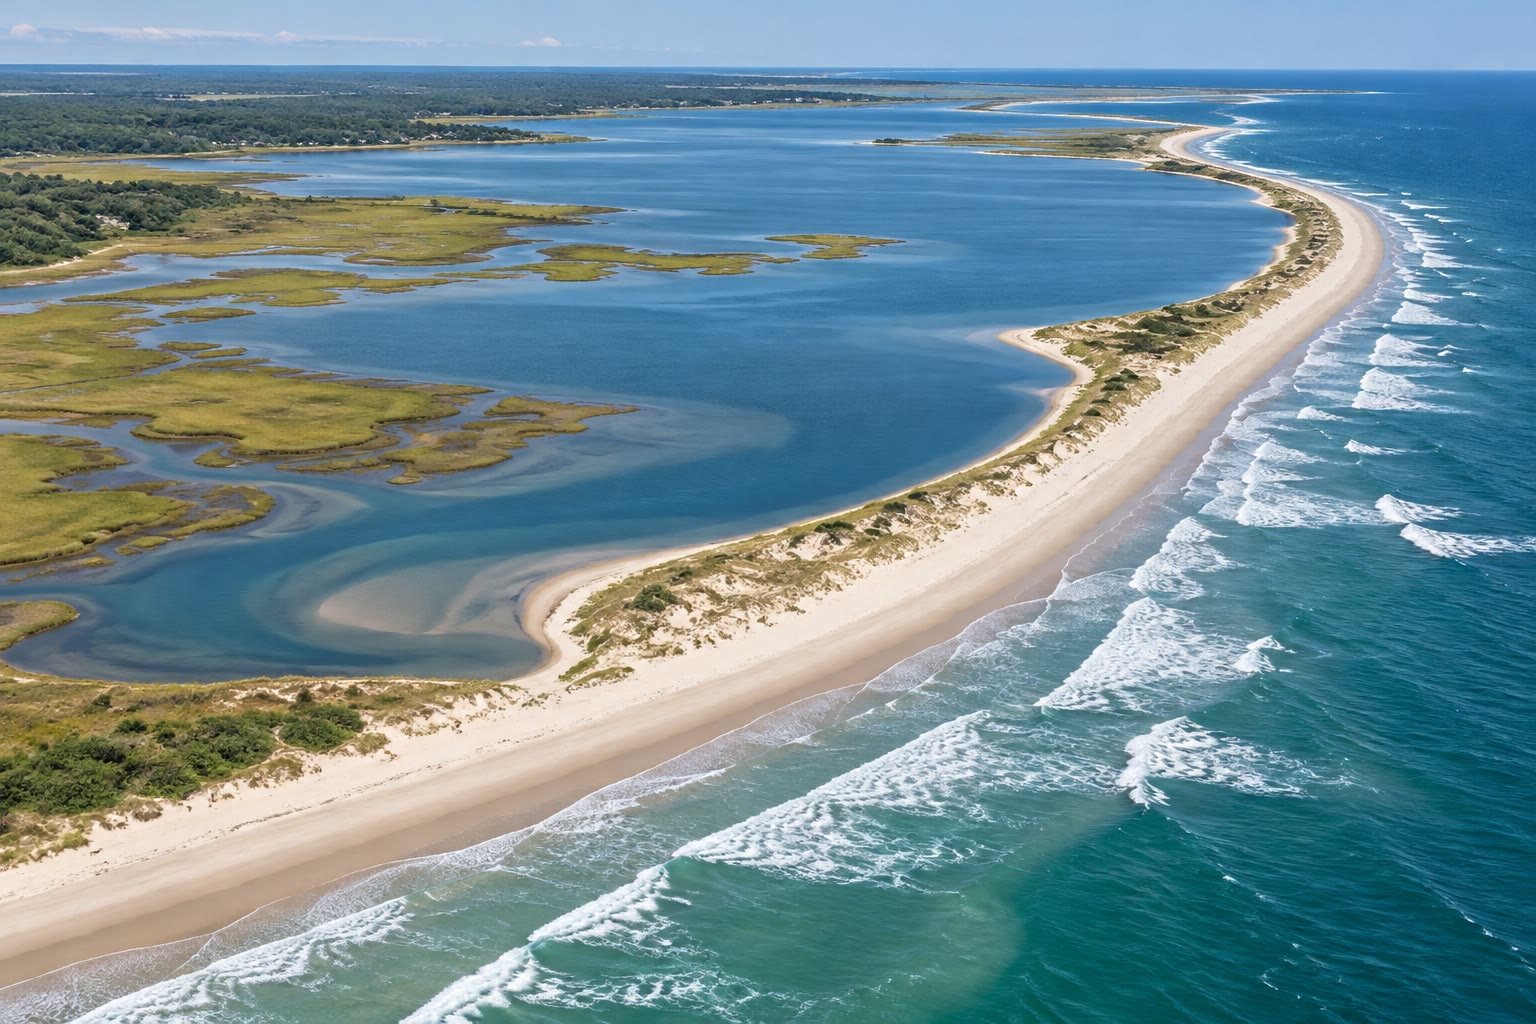
\includegraphics[width=\linewidth]{images/book1/ai/g9-spit-aerial.jpg}
\end{minipage}\hfill
\begin{minipage}[c]{0.46\linewidth}\raggedright
{\small \omterm{def:g9:landforms:beach}{لسان رملي} عبر مدخل خليج، كما يُرى من طائرة منخفضة (رسم توضيحي،
لا مكان حقيقي). تتكسر الأمواج على شاطئه المواجه \omterm{def:g2:water-on-earth:ocean}{للبحر}؛ وخلفه ماء هادئ
ومستنقعات ملحية.}
\end{minipage}
\label{fig:g9:landforms:spit-ai}
\end{omfigure}

\section{أشكال تضاريسية يصنعها الذوبان: الكارست}

ماء \omterm{def:g4:clouds-rain-snow:precipitation}{المطر} ليس ماءً نقيًا. فهو حين يسقط عبر الهواء ثم يتسرب عبر التربة،
يأخذ ثاني أكسيد الكربون، فيصير حمضيًا قليلًا. وهذا الحمض الضعيف يفعل
ببطء ما تفعله قطرة الحمض المخفف بسرعة بقطعة من الحجر الجيري: يذيب
\omterm{def:g3:stones-pebbles-sand:rock}{الصخر}. والحجر الجيري مليء بالشقوق، على طول طبقاته وعبرها. فيتسرب الماء
فيها ويوسعها، مليمترًا بعد مليمتر، على مدى آلاف
السنين.
% ledger: usgs:sinkholes, nps:karst

\begin{definition}[الكارست والكهف والبالوعة]\label{def:g9:landforms:karst}
\emph{الكارست}\index{كارست} \omterm{def:g1:landscapes-around-us:landscape}{منظر} طبيعي شكّله ماء يذيب \omterm{def:g3:stones-pebbles-sand:rock}{صخرًا} قابلًا
للذوبان، هو الحجر الجيري في أغلب الأحيان. وتميل \omterm{def:g1:landscapes-around-us:water}{الأنهار} فيه إلى الاختفاء
تحت الأرض ثم الخروج من جديد ينابيعَ. و\emph{الكهف}\index{كهف} فراغ طبيعي
تحت الأرض يتسع لدخول إنسان، أذابه الماء على طول شقوق \omterm{def:g3:stones-pebbles-sand:rock}{الصخر}.
و\emph{البالوعة}\index{بالوعة} تجويف أو ثقب في سطح الأرض، يتكوّن حيث يذوب
\omterm{def:g3:stones-pebbles-sand:rock}{الصخر} الذي تحته أو حيث ينهار سقف
كهف.
\end{definition}
% ledger: nps:karst, usgs:sinkholes

\begin{omfigure}
\begin{tikzpicture}[x=0.9cm, y=0.9cm, font=\footnotesize, >={Stealth[length=2mm]}]
  \pic (B) at (0,0) {blockdiagram={10}{4}{4}};
  % top face: grassland
  \fill[green!25!black!18] (B-ftl) -- (B-ftr) -- (B-btr) -- (B-btl) -- cycle;
  % right face
  \fill[omLithLime!70] (B-fbr) -- (B-bbr) -- (B-btr) -- (B-ftr) -- cycle;
  % front face: limestone layers
  \fill[omLithLime] (B-fbl) rectangle (B-ftr);
  \foreach \y in {0.8,1.6,2.4,3.2} \draw[black!35] (0,\y) -- (10,\y);
  \foreach \x/\y in {1.2/0.8, 3.1/1.6, 4.6/0, 6.8/2.4, 8.3/0.8, 2.2/2.4, 9.1/2.4, 5.6/3.2}
    \draw[black!35] (\x,\y) -- ++(0,0.8);
  % soil
  \fill[brown!45] (0,3.8) rectangle (10,4);
  % sinkhole on the top face and in the front face
  \fill[green!25!black!35] (3.0,4.45) ellipse (0.7 and 0.22);
  \fill[white] (2.3,4) -- (3.7,4) -- (3.25,3.45) -- (2.75,3.45) -- cycle;
  \fill[green!25!black!30] (2.3,4) -- (3.7,4) -- (3.25,3.45) -- (2.75,3.45) -- cycle;
  \draw[black!60] (2.3,4) -- (2.75,3.45) -- (3.25,3.45) -- (3.7,4);
  % shaft from sinkhole to cave
  \fill[white] (2.85,3.45) -- (3.15,3.45) -- (3.35,2.0) -- (3.05,2.0) -- cycle;
  \draw[black!60] (2.85,3.45) -- (3.05,2.0) (3.15,3.45) -- (3.35,2.0);
  % cave
  \fill[white] (2.6,2.1) .. controls (3.5,2.35) and (5.5,2.3) .. (6.6,1.9)
     .. controls (7.4,1.6) and (7.6,1.2) .. (7.2,1.0)
     .. controls (6.0,0.85) and (4.0,1.0) .. (3.0,1.2)
     .. controls (2.3,1.35) and (2.1,1.9) .. (2.6,2.1) -- cycle;
  \draw[black!70] (2.6,2.1) .. controls (3.5,2.35) and (5.5,2.3) .. (6.6,1.9)
     .. controls (7.4,1.6) and (7.6,1.2) .. (7.2,1.0)
     .. controls (6.0,0.85) and (4.0,1.0) .. (3.0,1.2)
     .. controls (2.3,1.35) and (2.1,1.9) .. (2.6,2.1);
  % underground stream at the cave floor
  \fill[omRiver!60] (3.0,1.2) .. controls (4.0,1.0) and (6.0,0.85) .. (7.2,1.0) -- (7.1,1.12)
     .. controls (6.0,1.0) and (4.0,1.12) .. (3.1,1.3) -- cycle;
  % stalactites and stalagmites
  \foreach \x/\l in {4.2/0.35, 4.5/0.22, 4.9/0.4, 5.3/0.25, 5.8/0.3}
    \fill[black!45] (\x-0.07,2.22) -- (\x+0.06,2.22) -- (\x,2.22-\l) -- cycle;
  \foreach \x/\l in {4.9/0.3, 5.8/0.25}
    \fill[black!45] (\x-0.12,0.95) -- (\x+0.12,0.95) -- (\x,0.95+\l) -- cycle;
  % disappearing stream on the top face
  \draw[omRiver, line width=1.2pt] (7.4,4.85) .. controls (6.9,4.5) and (6.4,4.4) .. (6.0,4.25);
  \fill[black!70] (6.0,4.25) circle (0.07);
  \draw[omRiver, dashed, thick] (6.0,4.0) -- (6.4,2.1);
  % spring on the right face
  \draw[omRiver, line width=1.2pt, ->] (10.2,1.2) .. controls (10.8,1.1) and (11.2,0.7) .. (11.6,0.5);
  % rain with carbon dioxide
  \foreach \x in {0.6,1.2,1.8} \draw[->, omRiver] (\x,5.6) -- ++(-0.15,-0.7);
  \draw[->, omRiver, dashed] (1.0,3.9) -- (1.2,1.7);
  % outline
  \draw[black!70] (B-fbl) rectangle (B-ftr);
  \draw[black!70] (B-ftl) -- (B-btl) -- (B-btr) -- (B-ftr) (B-btr) -- (B-bbr) -- (B-fbr);
  % labels
  \node[anchor=south, align=center] at (1.2,5.6) {المطر يأخذ ثاني أكسيد\\الكربون: حمضي قليلًا};
  \node[anchor=east, align=right] at (-0.1,1.6) {الماء يوسع\\الشقوق};
  \draw[black!70] (-0.05,1.6) -- (1.1,2.0);
  \node[anchor=south] at (3.0,5.2) {بالوعة};
  \draw[black!70] (3.0,5.2) -- (3.0,4.55);
  \node[anchor=south, align=center] at (7.6,5.3) {جدول يختفي\\تحت الأرض};
  \draw[black!70] (7.0,5.3) -- (6.1,4.35);
  \node[anchor=north, align=center] at (5.0,-0.1) {كهف: الهوابط تتدلى من السقف\\والصواعد ترتفع من الأرض};
  \draw[black!70] (5.0,-0.1) -- (5.0,1.4);
  \node[anchor=west, align=left] at (11.6,0.6) {ينبوع};
  \node[anchor=west] at (11.9,3.4) {حجر جيري};
\end{tikzpicture}

{\small \omterm{def:g1:landscapes-around-us:landscape}{منظر} كارستي (رسم تخطيطي، ليس بمقياس رسم). يتسرب ماء حمضي قليلًا
عبر شقوق الحجر الجيري ويوسعها؛ وتحفر الجداول الجوفية كهوفًا؛ وينهار سقف
\omterm{def:g9:landforms:karst}{كهف} فتنفتح \omterm{def:g9:landforms:karst}{بالوعة}؛ ويختفي جدول في ثقب ثم يخرج من جديد ينبوعًا في مكان
أخفض.}
% ledger: nps:karst, usgs:sinkholes, nps:speleothems
\label{fig:g9:landforms:karst}
\end{omfigure}

في \omterm{def:g9:landforms:karst}{الكهف}، يمكن أن يجري الذوبان في الاتجاه المعاكس. فقطرة الماء المتسربة
من السقف تحمل حجرًا جيريًا مذابًا. وحين تلاقي هواء \omterm{def:g9:landforms:karst}{الكهف}، تطلق بعض ثاني
أكسيد الكربون الذي فيها، فيخرج غشاء رقيق من الكالسيت من الماء حول
القطرة. وقطرة بعد قطرة، ينمو أنبوب أجوف من السقف، ثم يغلظ فيصير
\emph{هابطة كلسية}\index{هابطة كلسية}، تتدلى كقطعة جليد. وحيث تسقط
القطرات، يبني باقي الكالسيت \emph{صاعدة كلسية}\index{صاعدة كلسية} ترتفع
من الأرض. وحين تلتقيان، تصنعان
عمودًا.
% ledger: nps:speleothems

\begin{omfigure}
\begin{minipage}[c]{0.5\linewidth}\centering
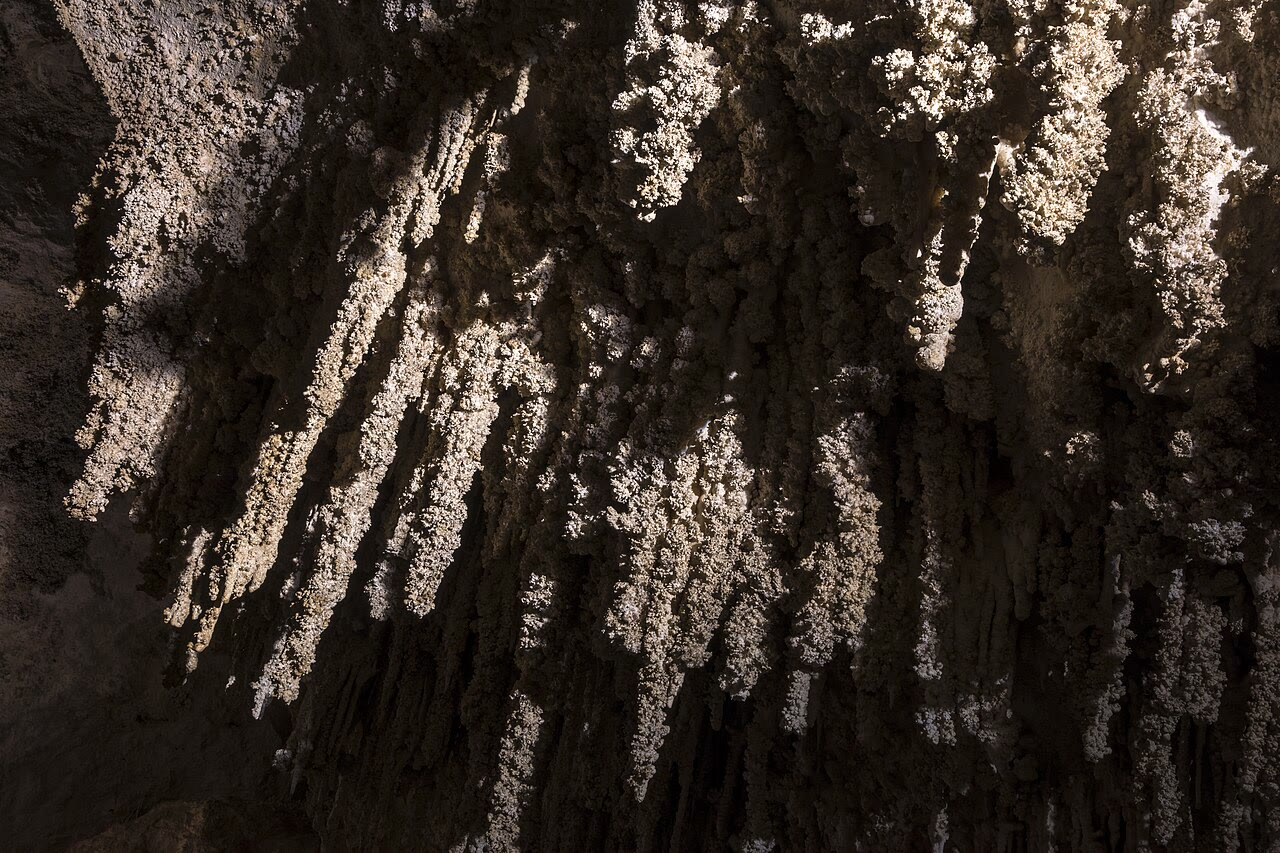
\includegraphics[width=\linewidth]{images/book1/g9-stalactites.jpg}
\end{minipage}\hfill
\begin{minipage}[c]{0.46\linewidth}\raggedright
{\small هوابط تتدلى تحت كتلة كبيرة من \omterm{def:g3:stones-pebbles-sand:rock}{الصخر} في \omterm{def:g9:landforms:karst}{كهف} كارلسباد، نيومكسيكو،
وهو \omterm{def:g9:landforms:karst}{كهف} أذابه الماء في الحجر الجيري. نمت كل منها قطرةً قطرةً من ماء
يتسرب عبر \omterm{def:g3:stones-pebbles-sand:rock}{الصخر} الذي فوقها. دائرة المتنزهات الوطنية الأمريكية، 2018
(ملك عام، عبر ويكيميديا كومنز).}
\end{minipage}
% ledger: commons:carlsbad-stalactites, nps:speleothems
\label{fig:g9:landforms:stalactites}
\end{omfigure}

تحوي بلاد \omterm{def:g9:landforms:karst}{الكارست} كثيرًا من الماء تحت الأرض، لكنه يجري بسرعة عبر الشقوق
المفتوحة ولا يكاد يُرشَّح: فكل ما يُسكب على الأرض قد يبلغ ينبوعًا بسرعة.
وحيث ذاب \omterm{def:g3:stones-pebbles-sand:rock}{الصخر} الذي تحتها، قد تهبط الأرض أو تنهار: وحيث يعيش الناس، قد
تبتلع \omterm{def:g9:landforms:karst}{بالوعة} تنفتح فجأة طرقًا
وبيوتًا.
% ledger: nps:karst, usgs:sinkholes

\section{قراءة منظر طبيعي}

كل \omterm{def:g1:landscapes-around-us:landform}{شكل تضاريسي} دليل. فشكله يقول أي عامل صنعه؛ والعامل يقول أي عملية
كانت تعمل، أهي \omterm{def:g5:water-shapes-the-land:erosion}{التعرية} أم \omterm{def:g5:water-shapes-the-land:deposition}{الترسيب}؛ والعملية كثيرًا ما تقول شيئًا عن
\omterm{def:g3:stones-pebbles-sand:rock}{الصخر} أو المواد المفككة التي تحته.

\begin{method}[قراءة شكل تضاريسي]
\begin{enumerate}
  \item \textbf{الشكل.} صِف \omterm{def:g1:landscapes-around-us:landform}{الشكل التضاريسي}: حافة، أو تجويف، أو واجهة
        شديدة الانحدار، أو رف مستوٍ؛ وحجمه؛ وإلى أين يتجه.
  \item \textbf{العامل والعملية.} قرّر أي عامل صنعه (\omterm{def:g1:landscapes-around-us:water}{نهر}، أو جليد، أو
        ريح، أو \omterm{def:g2:water-on-earth:ocean}{بحر}، أو ماء مذيب) وهل حُفر (\omterm{def:g5:water-shapes-the-land:erosion}{تعرية}) أم بُني
        (\omterm{def:g5:water-shapes-the-land:deposition}{ترسيب}).
  \item \textbf{المادة.} قل مما يتكوّن، أو ما يُرجَّح أن يكون \omterm{def:g3:stones-pebbles-sand:rock}{الصخر} الذي
        تحته: \omterm{def:g3:stones-pebbles-sand:sand}{رمل} مفكك، أو \omterm{def:g3:stones-pebbles-sand:pebble}{حصى}، أو حجر جيري، أو \omterm{def:g3:stones-pebbles-sand:rock}{صخر} صلب أو طري.
\end{enumerate}
\end{method}

\begin{center}
{\small
\begin{tabular}{|>{\raggedright\arraybackslash}p{4.6cm}|>{\raggedright\arraybackslash}p{2.6cm}|>{\raggedright\arraybackslash}p{2.2cm}|>{\raggedright\arraybackslash}p{2.6cm}|}
\hline
الشكل & العامل & العملية & المادة \\
\hline
\omterm{def:g1:landscapes-around-us:landform}{تلال} رملية هلالية الشكل & الريح & \omterm{def:g5:water-shapes-the-land:deposition}{ترسيب} & \omterm{def:g3:stones-pebbles-sand:sand}{رمل} مفكك \\
واجهة صخرية قائمة فوق رف صخري مستوٍ & \omterm{def:g2:water-on-earth:ocean}{البحر} & \omterm{def:g5:water-shapes-the-land:erosion}{تعرية} & \omterm{def:g3:stones-pebbles-sand:rock}{صخر} (\omterm{def:g3:stones-pebbles-sand:rock}{الصخر} الطري يتراجع بسرعة) \\
حافة ضيقة من \omterm{def:g3:stones-pebbles-sand:sand}{الرمل} عبر خليج & \omterm{def:g2:water-on-earth:ocean}{البحر} (\omterm{def:g9:landforms:beach}{الانجراف الساحلي}) & \omterm{def:g5:water-shapes-the-land:deposition}{ترسيب} & \omterm{def:g3:stones-pebbles-sand:sand}{رمل} أو \omterm{def:g3:stones-pebbles-sand:pebble}{حصى} \\
تجاويف في الحقول، وجداول تختفي & ماء مذيب & ذوبان & حجر جيري \\
\omterm{def:g8:ice-on-earth:glacial-landforms}{وادٍ على شكل حرف U} & الجليد & \omterm{def:g5:water-shapes-the-land:erosion}{تعرية} & أي \omterm{def:g3:stones-pebbles-sand:rock}{صخر} \\
مروحة من \omterm{def:g3:stones-pebbles-sand:sand}{الوحل} عند \omterm{def:g5:water-shapes-the-land:source-mouth}{مصب} \omterm{def:g1:landscapes-around-us:water}{نهر} & \omterm{def:g1:landscapes-around-us:water}{النهر} & \omterm{def:g5:water-shapes-the-land:deposition}{ترسيب} & \omterm{def:g3:stones-pebbles-sand:sand}{وحل} \omterm{def:g3:stones-pebbles-sand:sand}{ورمل} \\
\hline
\end{tabular}}
\end{center}

\begin{example}[نزهة على هضبة]
على هضبة عالية معشوشبة، لا يوجد أي جدول، مع أن \omterm{def:g4:clouds-rain-snow:precipitation}{المطر} يهطل كثيرًا.
والحقول منقطة بتجاويف مستديرة عرضها بضعة أمتار، وفي \omterm{def:g1:landscapes-around-us:landform}{الوادي} تحتها ينبثق
\omterm{def:g6:water-underground:spring}{ينبوع} قوي من أسفل واجهة صخرية.
\emph{الشكل}: تجاويف، ولا جداول على السطح، \omterm{def:g6:water-underground:spring}{وينبوع} في مكان أخفض.
\emph{العامل والعملية}: ماء يذيب \omterm{def:g3:stones-pebbles-sand:rock}{الصخر} ويجري تحت الأرض.
\emph{المادة}: الهضبة على الأرجح حجر جيري، والتجاويف \omterm{def:g9:landforms:karst}{بالوعات}. ولو وضع
المعلم قطرة من حمض مخفف على قطعة مفككة من \omterm{def:g3:stones-pebbles-sand:rock}{الصخر}،
لفارت.
\end{example}
% ledger: nps:karst, usgs:sinkholes

\section{تمارين}

\begin{exercise}[$\star$]\label{exo:g9:landforms:1}
أي عامل صنع كل \omterm{def:g1:landscapes-around-us:landform}{شكل تضاريسي}: الريح، أم \omterm{def:g2:water-on-earth:ocean}{البحر}، أم \omterm{def:g1:landscapes-around-us:water}{نهر}، أم الجليد، أم ماء
يذيب \omterm{def:g3:stones-pebbles-sand:rock}{الصخر}؟ (أ) \omterm{def:g1:landscapes-around-us:landform}{تلة} رملية هلالية الشكل في \omterm{def:g5:weather-and-climate:desert}{صحراء}. (ب) \omterm{def:g9:landforms:karst}{كهف} مليء بالهوابط.
(ج) حافة طويلة من \omterm{def:g3:stones-pebbles-sand:pebble}{الحصى} عبر مدخل خليج. (د) \omterm{def:g8:ice-on-earth:glacial-landforms}{وادٍ على شكل حرف U} في
نهايته \omterm{def:g8:ice-on-earth:glacial-landforms}{ركام جليدي}. (ه) واجهة طباشيرية قائمة عند قاعدتها رف صخري مستوٍ.
(و) \omterm{def:g5:water-shapes-the-land:delta}{دلتا}.
\end{exercise}

\begin{exercise}[$\star$]\label{exo:g9:landforms:2}
أعطِ الكلمة المناسبة لكل وصف. (أ) الارتفاع البطيء \omterm{def:g3:stones-pebbles-sand:rock}{لصخور} منطقة ولأرضها.
(ب) الجانب الشديد الانحدار من \omterm{def:g9:landforms:dune}{الكثيب}، البعيد عن الريح. (ج) ثقب في
الأرض يتكوّن حيث ذاب \omterm{def:g3:stones-pebbles-sand:rock}{الصخر} الذي تحته أو انهار سقف \omterm{def:g9:landforms:karst}{كهف}. (د) حركة \omterm{def:g3:stones-pebbles-sand:sand}{الرمل}
\omterm{def:g3:stones-pebbles-sand:pebble}{والحصى} على طول خط \omterm{def:g1:landscapes-around-us:water}{الساحل}. (ه) \omterm{def:g1:landscapes-around-us:landscape}{منظر} طبيعي شكّله ماء يذيب الحجر
الجيري.
\end{exercise}

\begin{exercise}[$\star$]\label{exo:g9:landforms:3}
صواب أم خطأ؟ صحّح الجمل الخاطئة. (أ) قرنا \omterm{def:g9:landforms:dune}{الكثيب} الهلالي يشيران نحو
الريح. (ب) منحدر \omterm{def:g9:landforms:dune}{الكثيب} المواجه للريح لطيف. (ج) يتحرك \omterm{def:g9:landforms:dune}{الكثيب} لأن الريح
ترفعه كله دفعة واحدة. (د) تتكوّن \omterm{def:g9:landforms:dune}{الكثبان} بسهولة أكبر حيث تنمو نباتات
قليلة.
\end{exercise}

\begin{exercise}[$\star$]\label{exo:g9:landforms:4}
رتّب مراحل تراجع \omterm{def:g9:landforms:cliff}{الجرف} البحري هذه. (أ) تكسر الأمواج الكتل الساقطة
وتحملها بعيدًا. (ب) تحفر الأمواج حزًّا عند قاعدة \omterm{def:g9:landforms:cliff}{الجرف}. (ج) صارت واجهة
\omterm{def:g9:landforms:cliff}{الجرف} الآن أبعد نحو اليابسة، والمصطبة المستوية التي أمامها أعرض قليلًا.
(د) يبرز \omterm{def:g3:stones-pebbles-sand:rock}{الصخر} الذي فوق الحزّ. (ه) يسقط
البروز.
\end{exercise}

\begin{exercise}[$\star\star$]\label{exo:g9:landforms:5}
% ledger: nps:whsa-migration (6 and 3 m a year)
من طائرة، تبدو \omterm{def:g9:landforms:dune}{الكثبان} الهلالية في \omterm{def:g5:weather-and-climate:desert}{صحراء} ما وقرونها كلها تشير إلى
الشرق. (أ) من أي اتجاه تهب الريح؟ (ب) في أي جانب من كل \omterm{def:g9:landforms:dune}{كثيب} يقع \omterm{def:g9:landforms:dune}{وجه
الانزلاق}؟ (ج) يمر طريق على بعد \qty{60}{m} شرق أحد \omterm{def:g9:landforms:dune}{الكثبان}. ويتحرك
\omterm{def:g9:landforms:dune}{الكثيب} \qty{6}{m} في السنة. بعد كم سنة تبلغ قاعدته الطريق؟ (د) يتحرك
\omterm{def:g9:landforms:dune}{كثيب} أكبر \qty{3}{m} فقط في السنة. لماذا تتحرك \omterm{def:g9:landforms:dune}{الكثبان} الأكبر ببطء
أكبر؟
\end{exercise}

\begin{exercise}[$\star\star$]\label{exo:g9:landforms:6}
% ledger: sdnp:birling, nt:birling-2014
تتراجع \omterm{def:g9:landforms:cliff}{الجروف} الطباشيرية \omterm{def:g1:landscapes-around-us:water}{لساحل} ما بما يصل إلى نحو \qty{1}{m} في السنة.
وفي شتاء 2014، فقدت ما تفقده عادةً في سبع سنوات، في شهرين فقط.
(أ) بمعدل \qty{1}{m} في السنة، كم يُفقد في سبع سنوات؟ (ب) الشهران أي
كسر من السنة؟ (ج) كم مرة أسرع من المعتاد تراجعت \omterm{def:g9:landforms:cliff}{الجروف} في هذين الشهرين؟
(د) اشرح، مستعينًا بالحزّ والبروز، لماذا يتراجع \omterm{def:g9:landforms:cliff}{الجرف} قفزات لا
بانتظام.
\end{exercise}

\begin{exercise}[$\star\star$]\label{exo:g9:landforms:7}
\omterm{def:g1:landscapes-around-us:water}{ساحل} مستقيم يمتد من الغرب إلى الشرق، \omterm{def:g2:water-on-earth:ocean}{والبحر} إلى جنوبه. وتأتي الأمواج من
الجنوب الغربي. (أ) في أي اتجاه يحمل \omterm{def:g9:landforms:beach}{الانجراف الساحلي} \omterm{def:g3:stones-pebbles-sand:sand}{الرمل}؟ (ب) ارسم
المسار المتعرج \omterm{def:g3:stones-pebbles-sand:pebble}{لحصاة} خلال ثلاث موجات، مسمّيًا الضربة الصاعدة على \omterm{def:g9:landforms:beach}{الشاطئ}
والضربة العائدة إلى أسفل. (ج) عند طرفه الشرقي ينعطف \omterm{def:g1:landscapes-around-us:water}{الساحل} شمالًا نحو
خليج. أي \omterm{def:g1:landscapes-around-us:landform}{شكل تضاريسي} يُرجَّح أن ينمو هناك؟ (د) لماذا يترسب \omterm{def:g3:stones-pebbles-sand:sand}{الوحل}
خلفه؟
\end{exercise}

\begin{exercise}[$\star\star$]\label{exo:g9:landforms:8}
(أ) ما الذي يجعل ماء \omterm{def:g4:clouds-rain-snow:precipitation}{المطر} حمضيًا قليلًا؟ (ب) لماذا توجد \omterm{def:g9:landforms:karst}{كهوف} في الحجر
الجيري ولا تكاد توجد في الغرانيت؟ (ج) لماذا تتبع \omterm{def:g9:landforms:karst}{الكهوف} الشقوق وطبقات
\omterm{def:g3:stones-pebbles-sand:rock}{الصخر}؟ (د) اذكر طريقتين لتكوّن \omterm{def:g9:landforms:karst}{البالوعة}.
\end{exercise}

\begin{exercise}[$\star\star$]\label{exo:g9:landforms:9}
(أ) اشرح لماذا يخرج الكالسيت من قطرة ماء معلقة في سقف \omterm{def:g9:landforms:karst}{كهف}. (ب) لماذا
لا يكون في الصواعد أنبوب أجوف، خلافًا للهوابط الفتية؟ (ج) افترض أن هابطة
نمت \qty{0.1}{mm} في السنة (معدل مخترع: فالمعدلات الحقيقية تتفاوت
كثيرًا). كم سنة استغرقت لتنمو \qty{30}{cm}؟ اكتب الجواب بالترميز
العلمي.
\end{exercise}

\begin{exercise}[$\star\star$]\label{exo:g9:landforms:10}
% ledger: usgs:himalaya, sdnp:birling
ارتفعت هضبة التبت نحو \qty{4600}{m} في نحو 10~ملايين سنة. (أ) احسب
متوسط \omterm{def:g9:landforms:uplift}{الرفع} بالأمتار في السنة، بالترميز العلمي، ثم بالمليمترات في
السنة. (ب) افترض أن \omterm{def:g5:water-shapes-the-land:erosion}{التعرية} تزيل \qty{0.2}{mm} في السنة من الهضبة (رقم
مخترع). بكم ترتفع الهضبة كل سنة؟ (ج) يتراجع \omterm{def:g9:landforms:cliff}{جرف} طباشيري نحو
\qty{1}{m} في السنة. كم مرة يكون ذلك أسرع من \omterm{def:g9:landforms:uplift}{رفع} (أ)؟ (د) لماذا
يستطيع \omterm{def:g9:landforms:uplift}{رفع} بطيء أن يبني هضبة عالية مع
ذلك؟
\end{exercise}

\begin{exercise}[$\star\star\star$]\label{exo:g9:landforms:11}
اقرأ كل \omterm{def:g1:landscapes-around-us:landscape}{منظر} بطريقة الفصل (الشكل، والعامل والعملية، والمادة). (أ) في بلد
جاف، صفوف طويلة من \omterm{def:g1:landscapes-around-us:landform}{التلال} الرملية، كل منها على شكل هلال، وجانبها الشديد
الانحدار يواجه الجنوب الشرقي. (ب) عند قاعدة \omterm{def:g9:landforms:cliff}{جرف} أبيض، يظهر عند الجزر
رف صخري مستوٍ مغطى بالأعشاب البحرية. (ج) على هضبة واسعة من \omterm{def:g3:stones-pebbles-sand:rock}{صخر} فاتح
اللون، يجري جدول عبر حقل ويختفي في ثقب؛ وينبثق \omterm{def:g6:water-underground:spring}{ينبوع} من جانب \omterm{def:g1:landscapes-around-us:landform}{وادٍ} على
بعد
\qty{2}{km}.
\end{exercise}

\begin{exercise}[$\star\star\star$]\label{exo:g9:landforms:12}
% ledger: nps:whsa-migration, nmt:barchan, nps:aeolian
في حقل \omterm{def:g9:landforms:dune}{كثبان}، تتحرك \omterm{def:g9:landforms:dune}{الكثبان} الصغيرة عند الطرف المواجه للريح حتى
\qty{6}{m} في السنة؛ وبعد ذلك بقليل، تتحرك \omterm{def:g9:landforms:dune}{الكثبان} التي ارتفاعها 6 إلى
\qty{10}{m} نحو \qty{3}{m} في السنة. ويعبر درب الحقل على بعد
\qty{45}{m} في اتجاه الريح من \omterm{def:g9:landforms:dune}{كثيب} من كل نوع. (أ) بعد كم سنة يبلغ كل
\omterm{def:g9:landforms:dune}{كثيب} الدرب؟ (ب) \omterm{def:g9:landforms:dune}{الكثبان} التي تدفعها رياح قوية قد تقطع أكثر من
\qty{100}{m} في السنة. كم يستغرق \omterm{def:g9:landforms:dune}{كثيب} كهذا ليقطع المسافة نفسها؟
(ج) اذكر طريقة واحدة لإبطاء \omterm{def:g9:landforms:dune}{الكثبان}، واشرح كيف تعمل.
\end{exercise}

\section{مسألة: الجرف والطريق الساحلي}

\begin{problem}[{مسألة نهاية الأسبوع --- طريق ساحلي يمتد خلف جرف
طباشيري يتراجع؛ والجواب الأخير هو السنة التي تبلغ فيها حافة الجرف
الطريق بالمعدل المقيس}]
\label{pb:g9:landforms:1}
% ledger: (invented region: exercise data, figdata/grade-9/cliff_retreat.py; the rate is kept within sdnp:birling, the storm winter recalls nt:birling-2014)
يمتد طريق ساحلي على طول قمة \omterm{def:g9:landforms:cliff}{جروف} طباشيرية. وكل بضع سنوات، يقيس فريق مسح
المسافة من الطريق إلى حافة \omterm{def:g9:landforms:cliff}{الجرف} على طول الخط نفسه، انطلاقًا من علامات
ثابتة مثبتة بعيدًا عن الحافة، لا عند الحافة نفسها أبدًا. وهذه
قياساتهم.

\begin{center}
{\small
\begin{tabular}{|l|c|c|c|c|c|c|c|}
\hline
السنة & 2004 & 2008 & 2012 & 2014 & 2016 & 2020 & 2024 \\
\hline
المسافة من الطريق إلى الحافة بالأمتار & 46.0 & 43.1 & 41.0 & 36.2 & 35.5 & 33.0 & 30.4 \\
\hline
\end{tabular}}
\end{center}

\noindent\textbf{الجزء الأول --- القياسات.}\par\nopagebreak
\begin{enumerate}[beginpenalty=10000]
  \item بكم مترًا اقتربت حافة \omterm{def:g9:landforms:cliff}{الجرف} من الطريق بين 2004
        و2024؟
  \item احسب متوسط معدل التراجع على مدى هذه السنوات العشرين، بالأمتار
        في السنة.
  \item بين أي مسحين تراجعت الحافة بأسرع ما يكون؟ احسب المعدل في تلك
        الفترة.
  \item كم مرة يكون أسرع من المتوسط؟ اقترح ما حدث في تلك
        الفترة.
\end{enumerate}

\begin{omfigure}
\begin{tikzpicture}
\begin{axis}[omrecord, width=11cm, height=4.6cm, xmin=2000, xmax=2070,
  ymin=0, ymax=50, xtick={2000,2010,...,2070}, ytick={0,10,...,50},
  x tick label style={/pgf/number format/1000 sep={}},
  xlabel={\foreignlanguage{arabic}{السنة}}, ylabel={\foreignlanguage{arabic}{المسافة إلى الطريق \babelsublr{(m)}}}]
  \addplot[omWarm, thick, mark=*, mark size=1.8pt] table[x=year, y=dist_m] {figdata/out/grade-9-cliff_retreat.dat};
\end{axis}
\end{tikzpicture}

{\small المسح: المسافة من الطريق الساحلي إلى حافة \omterm{def:g9:landforms:cliff}{الجرف} (بيانات
تمرين).}
\label{fig:g9:landforms:survey}
\end{omfigure}

\noindent\textbf{الجزء الثاني --- المعدل.}\par\nopagebreak
\begin{enumerate}[resume, beginpenalty=10000]
  \item اكتب متوسط المعدل بالسنتيمترات في السنة، ثم بالأمتار في
        القرن.
  \item على \omterm{def:g1:landscapes-around-us:water}{ساحل} طباشيري حقيقي، تتراجع \omterm{def:g9:landforms:cliff}{الجروف} بما يصل إلى نحو متر في
        السنة. هل تراجع هذا \omterm{def:g9:landforms:cliff}{الجرف} من الرتبة نفسها؟
  \item نُقلت مرةً منارة على \omterm{def:g1:landscapes-around-us:water}{ساحل} كهذا \qty{17}{m} إلى الوراء بعيدًا عن
        الحافة. بمتوسط معدل هذا \omterm{def:g9:landforms:cliff}{الجرف}، كم سنة من التراجع تمثل
        \qty{17}{m}؟
  \item لماذا يكون المعدل المقيس على مدى 20 سنة دليلًا أفضل إلى المستقبل
        من المعدل المقيس على مدى سنتين؟
\end{enumerate}

\noindent\textbf{الجزء الثالث --- الطريق.}\par\nopagebreak
\begin{enumerate}[resume, beginpenalty=10000]
  \item يجب نقل الطريق قبل أن تقترب الحافة منه إلى أقل من \qty{10}{m}.
        في أي سنة سيحدث ذلك، بالمعدل المتوسط؟
  \item لو ضاعفت شتاءات أكثر عصفًا المعدل، ففي أي سنة تبلغ الحافة
        الطريق؟
  \item لماذا يأخذ فريق المسح قياساته من علامات مثبتة بعيدًا عن
        الحافة؟
  \item بالمعدل المتوسط، في أي سنة تبلغ حافة \omterm{def:g9:landforms:cliff}{الجرف}
        الطريق؟
\end{enumerate}
\end{problem}
